\section{Introduction}
\subsection{Machine Learning Introduction}
Machine learning is an innovative application of artificial intelligence (AI) that empowers systems to learn and improve from experience autonomously without explicit programming. 

The learning process begins by observing or obtaining data, such as examples, direct experiences, or instructions, to identify patterns within the data and make informed decisions based on the provided examples. The ultimate goal is to enable computers to learn automatically, free from human intervention, and adapt their actions accordingly.

\subsubsection{Machine Learning algorithm}
\begin{itemize}
\item\textbf{Supervised Machine Learning: }This approach involves leveraging labeled examples from past data to predict the outcome of future events [2]. By analyzing a known training dataset to extract patterns and learn from it, the learning algorithm creates a model to generate predictions about output values. With sufficient training, the system can provide accurate predictions for new inputs. It can also compare its outputs with the correct ones to identify errors and adjust the model accordingly.
\begin{center}
    \begin{figure}[!htp]
        \centering
        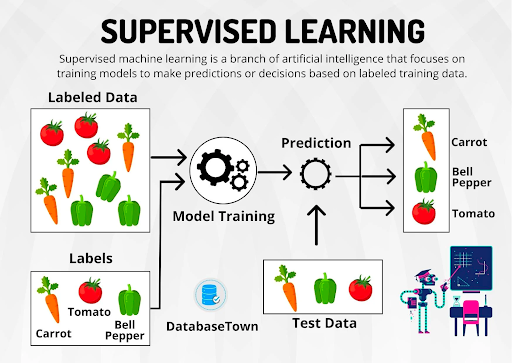
\includegraphics[width=0.8 \textwidth]{image/supervised_learning.png}
        \caption{Supervised learning}
        \label{subsection}
    \end{figure}
    \end{center}
\item\textbf{Unsupervised Machine Learning: } In scenarios where training data lacks labels or classification, unsupervised learning comes into play [3]. This approach focuses on inferring hidden structures within unlabeled data to develop a function that describes the data. While this method does not aim to determine specific outputs, it explores the data to uncover valuable insights and patterns.
\newline
For example (fig 1.2), the algorithm can extract the similar properties of fruits within a bag and group fruits with similar properties into different bags (same color or similar shape)

\begin{center}
    \begin{figure}[!htp]
        \centering
        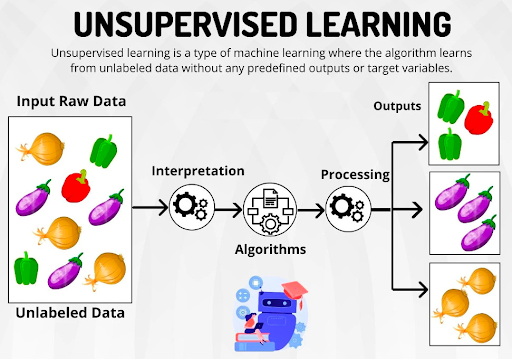
\includegraphics[width=0.8 \textwidth]{image/unsupervised_learning.png}
        \caption{Unsupervised learning}
        \label{subsection}
    \end{figure}
    \end{center}

\item\textbf{Semi-supervised machine learning:} Combining aspects of both supervised and unsupervised learning. This approach utilizes a mix of labeled and unlabeled data for training [4]. Typically, an algorithm works on a small amount of labeled data and a larger pool of unlabeled data. By incorporating this hybrid approach, learning accuracy can significantly improve. Also, obtaining labeled data is expensive and time-consuming, as the model can leverage the large pool of unlabeled data to improve its performance
\begin{center}
    \begin{figure}[!htp]
        \centering
        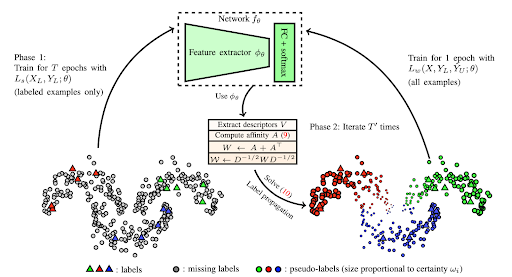
\includegraphics[width=0.8 \textwidth]{image/semi_supervised.png}
        \caption{semi-supervised learning}
        \label{subsection}
    \end{figure}
\end{center}

\item\textbf{Reinforcement learning:} This learning method involves an interactive process where an agent interacts with its environment, taking actions and receiving rewards [5]. Reinforcement learning is characterized by trial and error in making decisions and acquiring rewards. This approach enables machines and software agents to determine the optimal behavior within a specific context, maximizing their performance. Simple reward feedback guides the agent's learning process, known as the reinforcement signal. When combined with AI and cognitive technologies, machine learning becomes a powerful tool for processing vast amounts of information, yielding faster and more accurate results to identify the most profitable opportunities or potential risks. Reinforcement learning is commonly used in areas such as robotics, game-playing, and autonomous systems.
\begin{center}
    \begin{figure}[!htp]
        \centering
        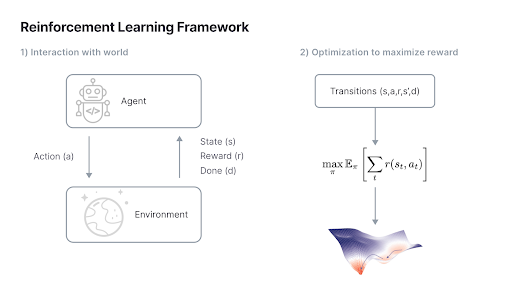
\includegraphics[width=0.8 \textwidth]{image/reinforcement_learning.png}
        \caption{Reinforcement learning}
        \label{subsection}
    \end{figure}
\end{center}
\end{itemize}

\subsection{Machine Learning in Everyday Applications}
\subsubsection{Virtual Personal Assistants}
Virtual personal assistants like Siri, Alexa, and Google Now have become popular examples of AI-driven applications. These assistants provide information and perform tasks when prompted using voice commands. By leveraging machine learning, they refine the information they provide based on user interactions and preferences. 
These assistants are integrated into platforms like Amazon Echo, Google Home, and smartphone software like Samsung Bixby.
\subsubsection{Predictive in communication}
Machine learning plays a crucial role in various aspects of communication. Traffic predictions rely on data from GPS navigation services to generate real-time traffic maps (for example, Google Maps) [6]. 
Machine learning algorithms can estimate areas prone to congestion by analyzing patterns and historical data. Online transportation networks also utilize machine learning to optimize routes, minimize detours, and predict demand, enhancing the efficiency and cost-effectiveness of shared mobility services [7].

\subsubsection{Video surveillance}
Machine learning revolutionizes video surveillance systems by enabling AI-powered detection of potential criminal activities. These systems can identify unusual behaviors, such as prolonged motionlessness or stumbling, and alert human attendants to prevent incidents. 
By continuously learning from data, machine learning enhances the accuracy and effectiveness of video surveillance, improving overall security [8].
\subsubsection{Social media services}
Machine learning underpins various features in social media platforms, enhancing user experiences and personalization. Examples include "People You May Know" recommendations, where machine learning analyzes user connections, profile visits, and shared interests to suggest potential friends. 
Face recognition algorithms leverage machine learning to identify and tag individuals in photos. Additionally, machine learning powers computer vision techniques that identify objects in images and recommend related content [9],
\subsubsection{Recommendation System}
Machine learning is instrumental in recommendation systems used by streaming platforms, e-commerce websites, and social media platforms. 
These systems analyze user preferences, browsing history, and behavior to suggest personalized content, products, or connections. By continuously learning from user feedback and interactions, recommendation systems improve their accuracy and provide tailored recommendations that cater to individual user preferences [10].

\subsection{Internet of Things}
\subsubsection{Introduction}
The Internet of Things (IoT) refers to a networked system where various physical objects are interconnected and accessible via the Internet. These objects, often called "things," can range from individuals with heart monitors to automobiles with sensors. 
Each object is assigned an IP address, enabling them to collect and transmit data over a network without manual intervention. By leveraging embedded technology, these objects can interact with their internal states or the surrounding environment, influencing their decisions. 

Typically, IoT's primary components are devices capable of connecting to the Internet and are divided into Sensors and actuators. Sensors are devices capable of detecting or measuring specific phenomena, collecting related data, and transmitting them to other entities (other IoT devices or application servers in the cloud). 
Some examples of IoT sensors include GPS devices, thermostats, and temperature sensors. To meet the cost-effectiveness requirements of IoT solutions, sensor nodes typically employ small-scale embedded systems, often utilizing 8-bit microcontrollers with limited storage capacity.
This design enables them to operate on battery power for extended periods, sometimes lasting years. Furthermore, a wide range of networking protocols allows sensor nodes to integrate seamlessly into existing infrastructures and diverse operational conditions. This flexibility greatly facilitates the deployment of IoT solutions across various domains [11].

On the other hand, Actuators are physical devices that can execute commands transmitted by a control center or act according to some programmed conditions to create a change in the surrounding environment [12].


\subsubsection{Applications of IoT}
IoT technology enhances mobility services, bolsters public safety, and automates city household systems. Within an area of smart city, one notable application is intelligent transportation, which focuses on optimizing road infrastructure and facilitating efficient route planning for drivers. 
It involves innovative solutions like smart traffic signals and sensors that monitor and manage traffic systems across the road network. By facilitating smoother traffic flow and reducing congestion, these technologies contribute to improved transportation experiences. 
However, the scope of smart city services extends beyond transportation. It encompasses various aspects of urban life, including public safety, environmental sustainability, efficient delivery of municipal services, smart grid systems, and integrating physical infrastructure with the digital realm. [13]

\begin{center}
    \begin{figure}[!htp]
        \centering
        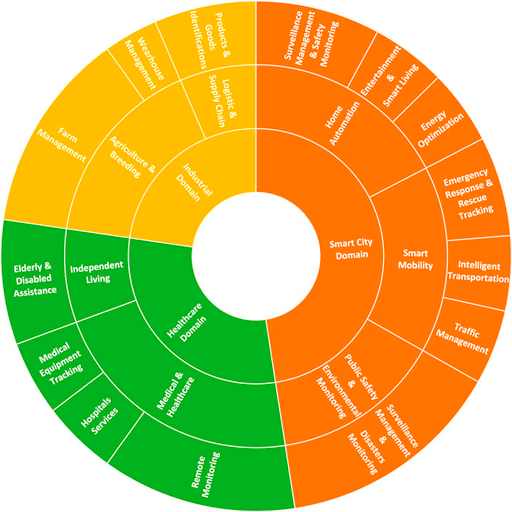
\includegraphics[width=0.8 \textwidth]{image/application_iot.png}
        \caption{Applications of IoT}
        \label{subsection}
    \end{figure}
    \end{center}

Home automation is another section (considered a sub-section of smart city), and control systems have significantly transformed our living environments. They have diverse applications within homes, including entertainment and smart living, surveillance, and safety management. Home automation refers to integrating IoT technology into a standard home environment to provide a secure and comfortable lifestyle. These systems rely on intelligent, self-adaptive mechanisms that analyze and evaluate user behaviors, predict future actions, and interact accordingly.  Home automation systems utilize image detection and facial recognition models embedded in an intelligent control system.
This control system is connected to sensors such as light, motion, water leak, smoke, and CCTV. These devices communicate with each other through a gateway distributed across a home area network. The home control system connects different subsystems collaborating to model user actions and gather environmental information, such as temperature, humidity, noise, visibility, and light intensity, to enhance learning.  For instance, lighting and AC temperature can be controlled and automated based on users' needs and movements within the home environment. Home automation research extends beyond energy optimization and encompasses health monitoring and security measures. 
By leveraging innovative IoT technologies, users can remotely access surveillance cameras within their homes through mobile devices. Additionally, stakeholders can employ door and window sensors to ensure home safety and security from a distance.

IoT has also expanded its application to the industrial sector. Industrial IoT harnesses the capabilities of IoT technology in the business and economic sectors to automate previously complex manual operations, meeting consumer demands while reducing production costs. Various industrial domains, including warehouse operations, logistics services, supply chain management, and agricultural breeding, can benefit from machine-to-machine (M2M) intercommunication, facilitating optimal industrial operations. For example, the application of communicating sensors in agricultural systems. 

\begin{center}
    \begin{figure}[!htp]
        \centering
        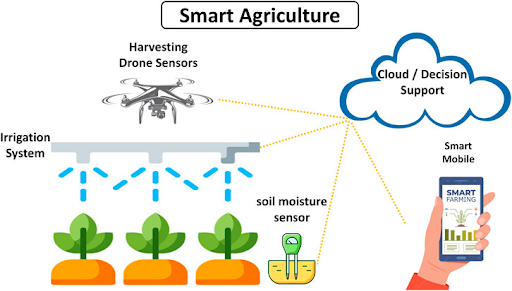
\includegraphics[width=0.8 \textwidth]{image/smart_argi.png}
        \caption{2.2 Smart agricultural system}
        \label{subsection}
    \end{figure}
    \end{center}
This system utilizes smart agriculture technology to monitor and analyze environmental parameters using sensors such as ZigBee, EnOcean, Z-wave, and ANT, which are specifically designed for soil moisture monitoring and harvesting. These sensors are automated to assess the plant's condition and gather relevant data through an IoT platform. Sensors utilize collected information to take appropriate actions, such as determining the optimal timing for irrigation by consulting a weather forecasting service available in the Cloud. It ensures the efficient utilization of water resources while maintaining crop health.
In the Healthcare domain, IoT also has a wide range of applications. IoT sensors and devices have transformed the landscape of portable and wearable medical devices, expanding their applications from fitness and wellness to medically qualified devices suitable for use in hospitals and healthcare facilities. This shift has facilitated the integration of remote patient monitoring (RPM) in healthcare settings, particularly for patients with chronic diseases. As a result, significant efforts are made to advance RPM systems by leveraging well-established IoT infrastructures and standards in the healthcare domain. These RPM systems aim to match or surpass the performance of existing monitoring and examination methods employed in hospitals and healthcare facilities.  For instance, continuous heart rate monitoring and immediate detection of irregular heartbeats traditionally required patients to be hospitalized or connected to devices like Holter monitors for long-term cardiac diagnosis. 
However, these setups limited patient mobility due to device size and the number of connected wires.

Furthermore, hospitals expended substantial resources on providing long-term cardiac monitoring, which was often unavailable, particularly in low or middle-income countries. 
Remote patient monitoring systems effectively address these challenges and reduce mortality rates associated with chronic diseases such as heart disease and diabetes. IoT platforms and devices have played a significant role in accelerating the development and integration of RPM systems into existing healthcare infrastructures. Consequently, a typical RPM implementation encompasses various services, including but not limited to data acquisition, tracking, communication, automated analysis, diagnoses, and notification systems.

\subsection{Neural Networks & Deep learning}
\subsubsection{Neural Networks & Deep learning introduction}
A neural network is a series of algorithms that aims to discover underlying relationships in a dataset by simulating the functioning of the human brain. Neural networks can adapt to changing input, generating optimal results without redesigning output criteria. 
This concept, rooted in artificial intelligence, is increasingly popular in developing intelligent systems.

In finance, neural networks are utilized in various processes such as time-series forecasting, algorithmic trading, securities classification, credit risk modeling, and constructing proprietary indicators and price derivatives.

Moreover, neural networks have been widely used for image recognition tasks such as object detection, image classification, and facial recognition. In natural language processing, it has shown remarkable performance in various tasks such as language translation, sentiment analysis, and text generation. 
Also, the application of neural networks has been demonstrated in speech recognition, autonomous vehicles, and medical diagnosis. 
The functioning of a neural network resembles that of the human brain's neural network. A "neuron" in a neural network is a mathematical function that collects and categorizes information based on a specific architecture. The network bears similarities to statistical methods like curve fitting and regression analysis [14].

A neural network consists of interconnected layers of nodes, where each node functions as a perceptron, similar to multiple linear regression. The perceptron passes the signal from multiple linear regression through an activation function, which can be nonlinear

In a multi-layered perceptron (MLP), perceptrons are organized into interconnected layers. The input layer receives input patterns, while the output layer provides classifications or output signals corresponding to the input patterns. 
For example, input patterns may consist of technical indicators for security, and potential outputs could be "buy," "hold," or "sell".

Hidden layers in the neural network adjust the input weightings until the network's margin of error is minimized. It is hypothesized that hidden layers extract significant features from the input data that have predictive power for the outputs. This process, known as feature extraction, serves a purpose similar to statistical techniques like principal component analysis [15].
\begin{center}
    \begin{figure}[!htp]
        \centering
        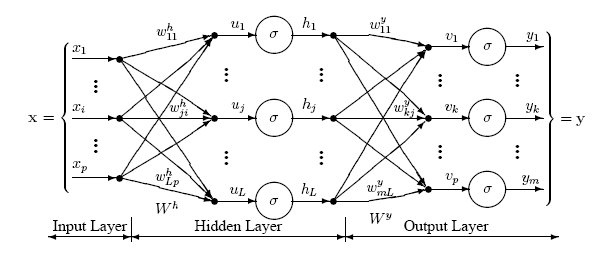
\includegraphics[width=0.8 \textwidth]{image/MLFN_with_weights.jpeg}
        \caption{Multi-layer perceptron}
        \label{subsection}
    \end{figure}
    \end{center}

A Deep Neural Network (DNN) is a type of artificial neural network (ANN) that consists of multiple layers between the input and output layers. The DNN employs various mathematical operations to transform the input into the desired output, accommodating both linear and non-linear relationships.

Deep learning is a specific function within the field of artificial intelligence (AI) that emulates the information processing and pattern recognition capabilities of the human brain. It falls under the umbrella of machine learning and involves the use of neural networks capable of unsupervised learning from unstructured or unlabeled data. It is also referred to as deep neural learning or deep neural network [15].

\subsubsection{Machine learning vs Deep learning}

\begin{center}
    \begin{figure}[!htp]
        \centering
        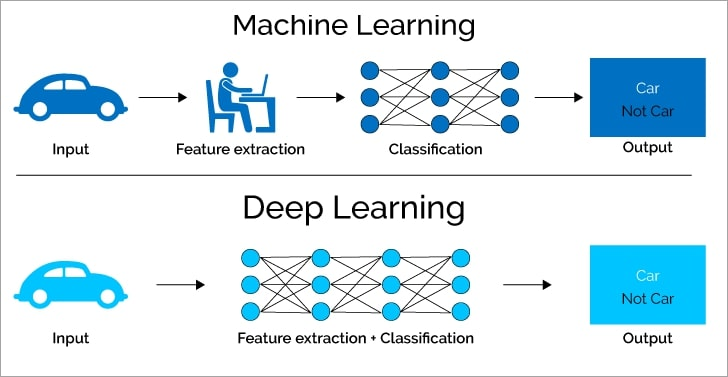
\includegraphics[width=0.8 \textwidth]{image/dnn_vs_ml.png}
        \caption{Deep learning vs Machine learning}
        \label{subsection}
    \end{figure}
    \end{center}

Deep neural networks are characterized by their deeply nested network architectures, typically consisting of multiple hidden layers. These networks employ advanced neurons that utilize operations like convolutions and multiple activations within a single neuron, going beyond the simple activation functions used in traditional artificial neural networks (ANNs). 
It enables deep neural networks to process raw input data and automatically learn representations relevant to the learning task. This capability is commonly referred to as deep learning. In contrast, simple ANNs (such as shallow autoencoders) and other machine learning (ML) algorithms like decision trees are considered part of shallow machine learning as they lack these functionalities. 
While some shallow ML algorithms are inherently interpretable by humans and are considered as white boxes, the decision-making process of most advanced ML algorithms is inherently untraceable unless explicitly explained, making them black boxes.

Deep learning (DL) excels in domains with large and high-dimensional datasets, making deep neural networks outperform shallow ML algorithms in tasks involving text, image, video, speech, and audio data processing. 
However, when dealing with low-dimensional data inputs, especially in scenarios with limited training data availability, shallow ML approaches can still produce superior result, 
which are often more interpretable compared to those generated by deep neural networks [16]. 

\subsubsection{Applications and challenges of AI in Internet of thing}
Several case studies have showcased the successful integration of Internet of Things (IoT) and machine learning technologies in various fields including smart cities such as improving the efficiency of urban services, and enhancing citizens' overall quality of life. 
Deep learning algorithms combined with video analysis have been identified as practical applications in smart cities. 
In one study, researchers developed an IoT system based on deep learning for remote monitoring and early detection of health issues in real time. 
The system exhibited impressive accuracy in identifying heart conditions, achieving a remarkable accuracy rate of 0.982 [17, 18].

However, deploying deep learning methodologies within IoT frameworks presents challenges and limitations. These challenges can be broadly categorized into ethical and privacy implications, scalability and resource constraints, and the ongoing need for research and development.
Integrating deep learning into IoT has significantly advanced security and efficiency in surveillance applications. IoT devices with deep learning capabilities, such as convolutional neural networks, can effectively analyze video streams to detect threats and anomalies, improving real-time monitoring and predictive insights.

Nevertheless, these applications face significant challenges, such as the need for extensive datasets and substantial computational power.
The scalability of deep learning models in the IoT poses a significant concern. IoT devices often have limited computational resources, making it challenging to deploy complex deep-learning models that require substantial data processing capabilities.
It is crucial to optimize these models for deployment on resource-constrained devices, necessitating innovative solutions that strike a balance between the computational demands of deep learning algorithms and the inherent limitations of IoT hardware. [19]
